Each graph shows a harmonic oscillation. Write it as $y(t) = A\cos(\omega t - \varphi_0)$ with $-\pi < \varphi_0 \le \pi$: what are the amplitude $A$, the period $T$ and the phase $\varphi_0$? Give the phase as a multiple of $\pi$.

\begin{abcliste}
\abc
\begin{center}
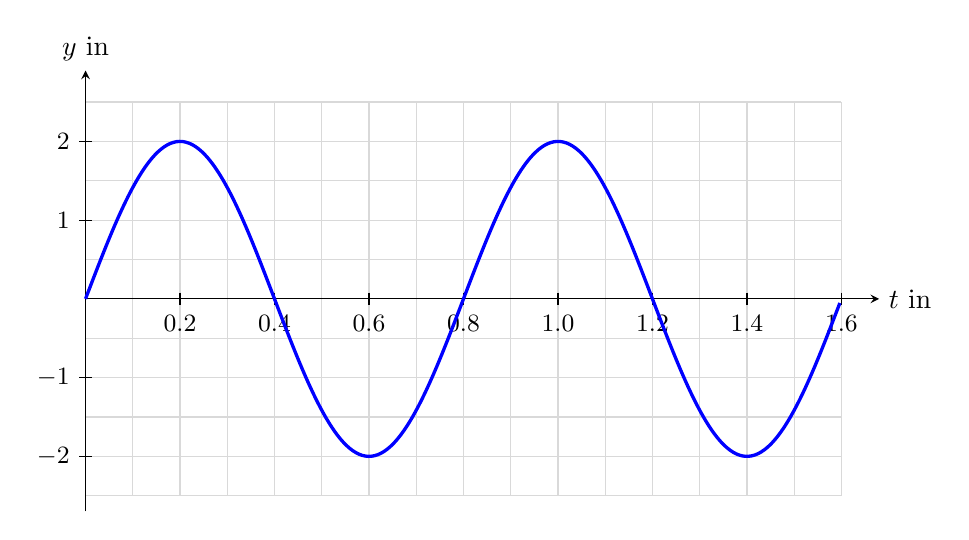
\begin{tikzpicture}[xscale=6, yscale=1, >=stealth]
 \draw[black!15] (0,-2.5) grid[xstep=0.1, ystep=0.5] (1.6,2.5);
 \draw[->] (0,0) -- (1.68,0) node[right] {$t$ in \si{\second}};
 \draw[->] (0,-2.7) -- (0,2.9) node[above] {$y$ in \si{\cm}};
 \foreach \xt in {0.2,0.4,0.6,0.8,1.0,1.2,1.4,1.6} \draw (\xt,0.08) -- (\xt,-0.08) node[below] {\small $\xt$};
 \foreach \yt in {-2,-1,1,2} \draw (0.013,\yt) -- (-0.013,\yt) node[left] {\small $\yt$};
 \draw[very thick, blue, domain=0:1.6, samples=241, smooth] plot (\x, {2*cos(450*\x - 90)});
\end{tikzpicture}
\end{center}

\abc
\begin{center}
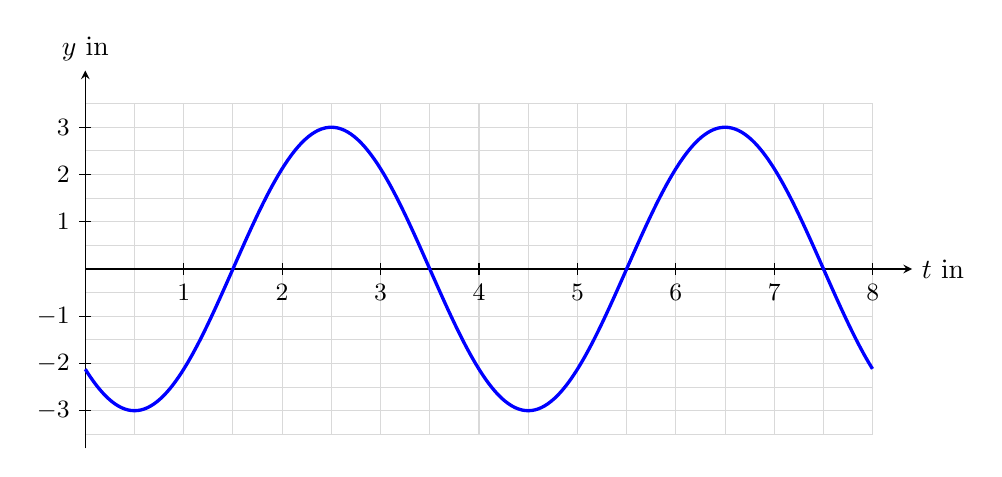
\begin{tikzpicture}[xscale=1.25, yscale=0.6, >=stealth]
 \draw[black!15] (0,-3.5) grid[xstep=0.5, ystep=0.5] (8,3.5);
 \draw[->] (0,0) -- (8.4,0) node[right] {$t$ in \si{\second}};
 \draw[->] (0,-3.8) -- (0,4.2) node[above] {$y$ in \si{\cm}};
 \foreach \xt in {1,2,3,4,5,6,7,8} \draw (\xt,0.13) -- (\xt,-0.13) node[below] {\small $\xt$};
 \foreach \yt in {-3,-2,-1,1,2,3} \draw (0.06,\yt) -- (-0.06,\yt) node[left] {\small $\yt$};
 \draw[very thick, blue, domain=0:8, samples=241, smooth] plot (\x, {3*cos(90*\x + 135)});
\end{tikzpicture}
\end{center}
\end{abcliste}
